\documentclass[12pt,a4paper]{article}
\usepackage[utf8]{inputenc}
\usepackage[a4paper, total={6in, 9in}]{geometry}
\usepackage{amsmath}
\usepackage{amsfonts}
\usepackage{amssymb}
\usepackage{graphicx}
\usepackage{fancyhdr}
\usepackage{float}
\usepackage[parfill]{parskip}
\begin{document}

\thispagestyle{empty}

\begin{center}
\LARGE\textbf{PHY408 Lab 0} \\
\vspace{5mm}
\Large Kevin Dang - 1003205079	
\end{center}

\vspace{5mm}

\section*{2 Integration Function}

\subsection*{Part 1}
Collaborators: None
\begin{figure}[H]
    \centering
    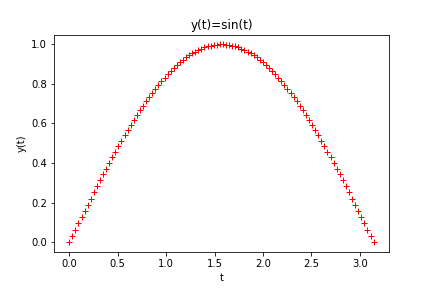
\includegraphics[width=0.7\textwidth]{fig1.png}
    \caption{$y(t) = \sin(t)$}
\end{figure}

The output $c$ value of $1.9998321638939935$ is close to what I expected for the integral, which is a value of 2 if the integral is computed manually.

To improve accuracy of the computation, we can increase $nt$, the number of samples. This would decrease the sample interval $dt$ so we are less likely to exclude area.

\newpage
\subsection*{Part 2}
Collaborators: None
\begin{figure}[H]
    \centering
    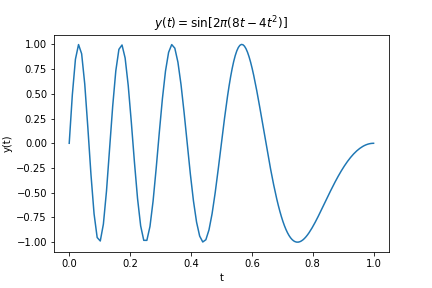
\includegraphics[width=0.7\textwidth]{fig2.png}
    \caption{$y(t) = \sin[2\pi(8t-4t^2)]$ \ (for $nt=50$)}
\end{figure}

$\int_0^1 \sin[2\pi(8t-4t^2)] = -0.10540213617112387$

\begin{figure}[H]
    \centering
    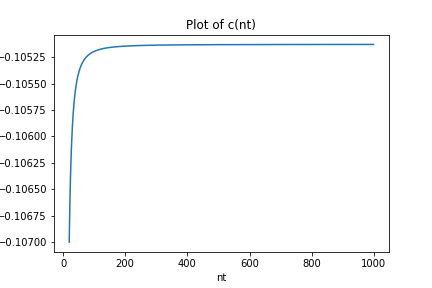
\includegraphics[width=0.7\textwidth]{fig3.png}
    \caption{$c(nt)$}
\end{figure}

As $nt$ increases, $c$ converges to $\int_0^1 \sin[2\pi(8t-4t^2)] = -0.10540213617112387$.

\newpage
\section*{3 Accuracy of Sampling}
Collaborators: Erich Fernandes
\begin{figure}[H]
    \centering
    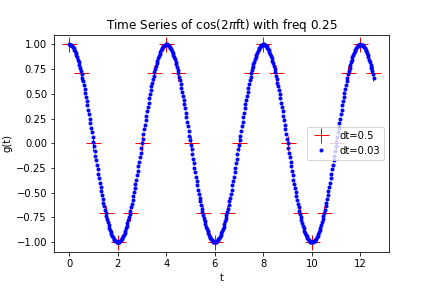
\includegraphics[width=0.7\textwidth]{fig4.png}
    \caption{Time Series of cos(0.5$\pi$t)}
\end{figure}

\begin{figure}[H]
    \centering
    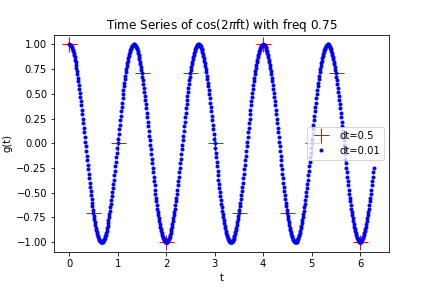
\includegraphics[width=0.7\textwidth]{fig5.png}
    \caption{Time Series of cos(1.5$\pi$t)}
\end{figure}

Q: \textit{For each frequency that you investigated, do you think the sampling time series is a fair representation of the original time series $g(t)$?}

A: The sampling time series is a fair representation of the original time series $g(t)$ at frequencies such as 0, 0.25, 0.5 and 1 hertz. The samples hit important points like the minima, maxima and points of inflection and they also have an apparent frequency that is equal to the true frequency. However when we get to larger frequencies like 0.75, 1.5, 2 hertz these sampling time series miss crucial points that define the original time series so they are not a good representation. In addition the apparent frequencies are not equal to the true frequency.

Q: \textit{What is the apparent frequency for the sampling time series?}

A: The apparent frequency for the sampling time series is in Table \ref{table:1} below. For example, if we have $f$ = 0.75 then the apparent frequency is 0.25, even though the true frequency is 0.75. This is because the samples occur N = 8 times per cycle so the frequency is 1/(N*dt) = 1/(8*0.5) = 0.25. \\

\begin{table}[H]
\centering
\begin{tabular}{|c|c|c|}
\hline
frequency & Points the series repeats itself (N) & apparent frequency  \\
\hline\hline
0 & N/A (flat line) & 0 \\
\hline
0.25 & 8 & 0.25  \\
\hline
0.5 & 4 & 0.5  \\
\hline
0.75 & 8 & 0.25 \\
\hline
1 & 2 & 1 \\
\hline
1.5 & 4 & 0.5 \\
\hline
2 & N/A (flat line) & 0 \\
\hline
\end{tabular}
\caption{Frequencies and Apparent Frequencies}
\label{table:1}
\end{table}

Q: \textit{Can you guess with a sampling interval of $dt=0.5$ , what is the maximum frequency $f$ of $g(t)$ such that it can be fairly represented by the discrete time series?}

A: I estimate the maximum frequency to be 0.5. This is because after the frequency goes beyond 0.5 the apparent frequency does not match the true frequency. 

\end{document}